\documentclass[english]{article}



\usepackage{graphicx}
\usepackage[hidelinks]{hyperref}
\usepackage{grffile}
\usepackage[T1]{fontenc}
\usepackage{babel}
\usepackage{float}
\usepackage{tabu}
\usepackage{ragged2e}
\usepackage{textcomp}
\usepackage{amstext}
\usepackage[final]{pdfpages}
\usepackage{caption}
\usepackage{color}


\graphicspath{{Pictures/}}


\begin{document}
	
	
	\begin{figure}[H]
		
\includegraphics[width=\linewidth]{teamphoto.jpg}
	\end{figure}

	\begin{figure}[H]
		
\includegraphics[width=\linewidth]{teamtitle.jpg}
	\end{figure}

	\begin{figure}[H]
		
\includegraphics[width=\linewidth]{documenttitle.jpg}
	\end{figure}

	\begin{figure}[H]
		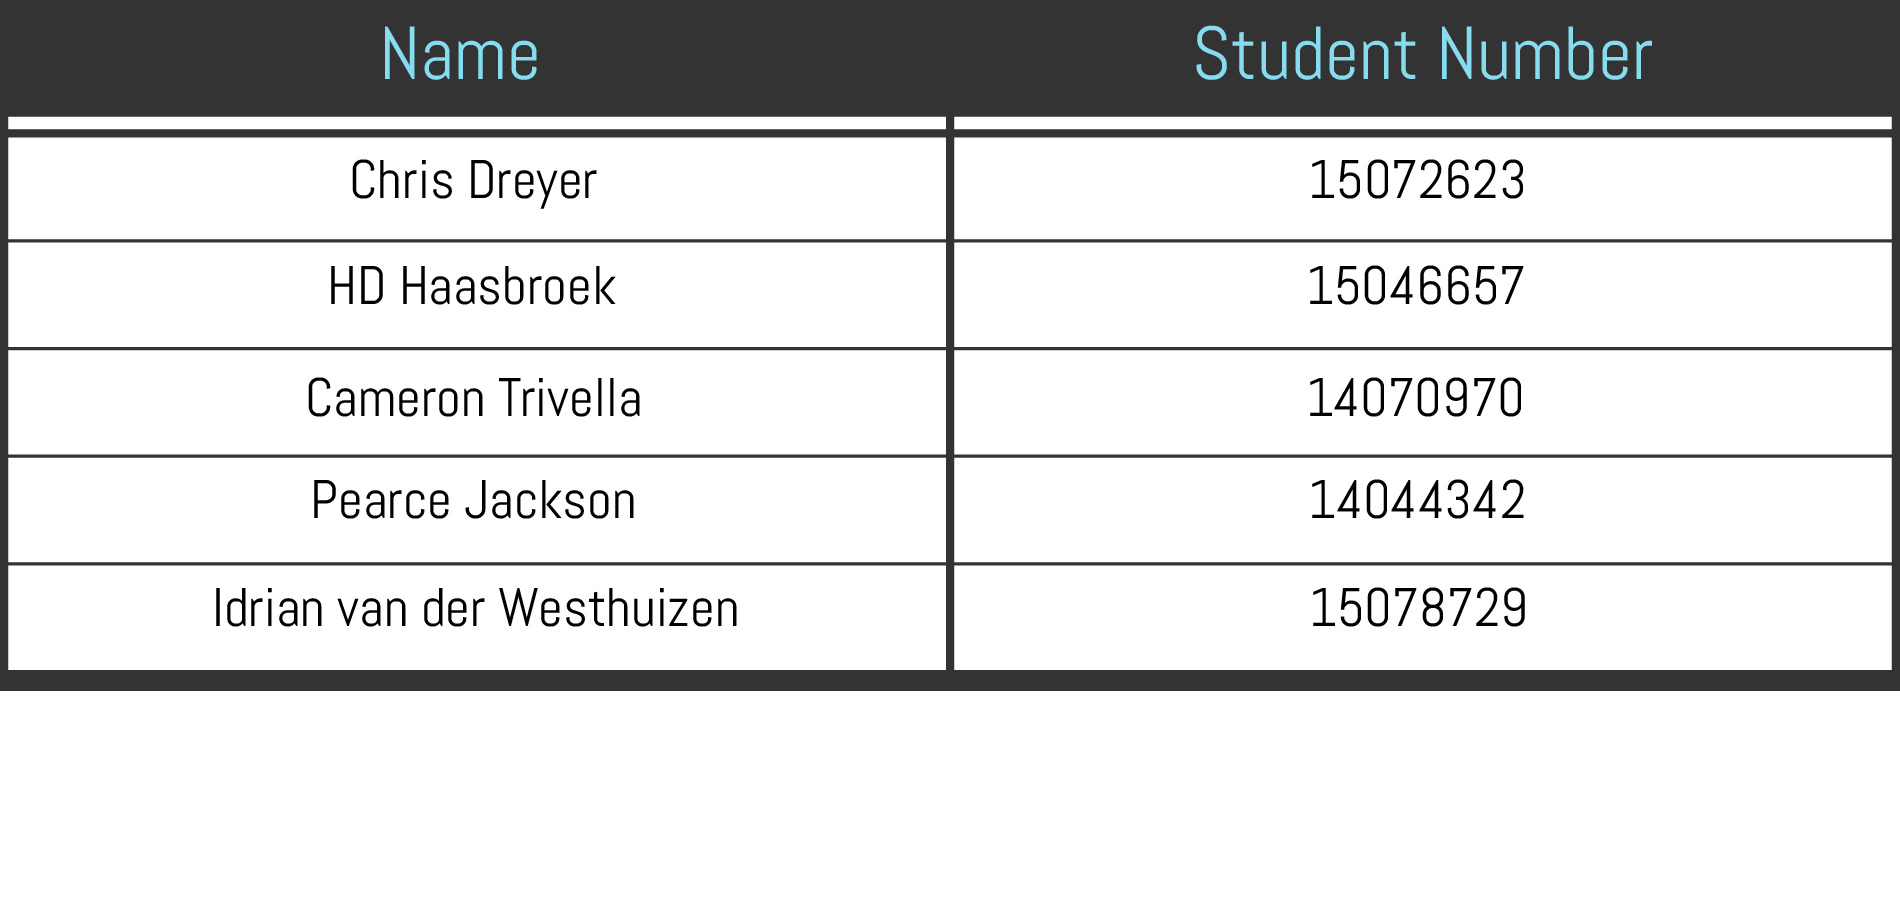
\includegraphics[width=\linewidth]{teamtable.jpg}
	\end{figure}
	
	\pagenumbering{gobble}
	\newpage
	\tableofcontents
	
	\pagenumbering{arabic}
	\newpage

	\section{Introduction}
	
		\subsection{Purpose}
		
		This SRS document aims to stipulate the requirements of the voxc.js library to aid in the development process and to ensure that a functional and usable product is delivered.
		
		\subsection{Product Scope}
		
		Voxc.js is meant to be an easy to use and easy to maintain JavaScript library, similar to how three.js is a library for WebGL. The purpose of the project is to provide users a way to import Voxel models into a webpage that would be using the Voxc.js library and ultimately texturing these Voxel models according to a rules file with a specified structure. The user will then be able to export the textured and rendered object.
		
		\subsection{References}
		
		\color{blue}
		\url{http://www.oskarstalberg.com/game/house/Index.html}
		\newline
		\\\url{https://voxel.codeplex.com/}
		\newline
		\\\url{https://pages.github.com/}
		\newline
		\\\url{http://threejs.org/}
		\newline
		\\\url{http://coffeescript.org/}
		\newline
		\\\url{http://es6-features.org/#Constants}
		\newline
		\\\url{http://www.typescriptlang.org/}
		\newline
		\\\url{http://www.codebelt.com/typescript/typescript-es6-modules-boilerplate/}
		\newline
		\\\url{http://giacomotag.io/typescript-webpack/}
		\color{black}
		
	\pagebreak
	
	\section{External Interface Requirements}
	
		\subsection{User Interfaces}
		
		\subsection{Software Interfaces}
		
		\subsection{Communications Interfaces}
		
	\pagebreak
	
	\section{System Features}
	
		\subsection{System Feature 1}
		
			 \subsubsection{Description and Priority}
			 
			 \subsubsection{Stimulus/Response Sequences}
			 
			 \subsubsection{Functional Requirements}
			 
	\pagebreak
	
	\section{Other Nonfunctional Requirements}
	
		\subsection{Performance Requirements}
		
		\subsection{Security Requirements}
		
		\subsection{Quality Requirements}
		
	\pagebreak
	
\end{document}